%%%% Input Codes %%%%   
% <mcode.sty> required

% \lstset{numbers=left,numberstyle= \tiny}
% \lstinputlisting[firstline=6, lastline=15]{/Users/name/Desktop/FILENAME.M}

% or:

%\lstset{numbers=left,numberstyle= \tiny}
%\begin{lstlisting}[xleftmargin=2em,xrightmargin=2em,aboveskip=1em]
%clc; clear all; close all;
%\end{lstlisting}

\section{Model Set-up}

Krusell\&Smith(1998) develop a computational algorithm to approximate the equilibrium. The main challenge is to compute the law of motion for the aggregate states.

Based on Luis's lecture slides, the infinitely lived consumers and only one good $y$ production function are:

\begin{align}
\begin{split}
E_0 \sum_{t=0}^{\infty} \beta^t \frac{c^{1-\sigma} - 1}{1 - \sigma} \\
y = z k^{\alpha}l^{1-\alpha}
\end{split}
\end{align}



\begin{enumerate}
\item Each worker supplies $\epsilon \bar{l}$ units of labor input, where $\epsilon$ is stochastic and can be 0 (unemployed) or 1 (employed). 

\item z is the stochastic shock to aggregate productivity with two possible realizations: $z_g$ (good) or $z_b$ (bad). The process is Markov with transition probability $\pi_{ss'}$.

\item $\pi_{ss' \epsilon \epsilon'}$ is the transition probability of the joint distribution.
\end{enumerate}

The household problem solves

\begin{align} \label{hhproblem}
\begin{split}
v(k,\epsilon; \Gamma ,z) &= \max_{c,k'} \{ \frac{c^{1-\sigma} - 1}{1 - \sigma} + \beta E [v(k',\epsilon'; \Gamma' ,z')| z, \epsilon]\} \\
\text{subject to} \\
& c + k' = r(\bar{k},\bar{l},z)k + w(\bar{k},\bar{l},z)\tilde{l}\epsilon + (1-\delta)k \\
& \Gamma' = H(\Gamma,z,z') \\
& k' \geq 0
\end{split}
\end{align}


and firms maximizing profits yield:

\begin{align} \label{firms}
\begin{split}
r(\bar{k},\bar{l},z) = \alpha z (\frac{\bar{k}}{\bar{l}})^{\alpha-1} \\
w(\bar{k},\bar{l},z) = (1-\alpha) z (\frac{\bar{k}}{\bar{l}})^{\alpha}
\end{split}
\end{align}


and the laws of motion of z and $\epsilon$, where decision rule is characterized by $f: k' = f(k,\epsilon; \Gamma, z)$

\textbf{Issue:} Need to keep track of the distribution $\Gamma$ (infinite dimensional object); the law of motion H is unknown.

\textbf{Solution Idea:} Approximate $\Gamma$ by moments and assume a functional form of H which maps moments to moments. In other words, they explore whether it is possible to approximate the distribution $\Gamma_t$ with a finite set of M moments, call it $$m = {m_1,m_2, \dots, m_M}$$ with law of motion for the moments $m' =H_M (\Gamma, z,z')$.

\subsection{{\color{red}Basic Algorithm Steps}}
\begin{enumerate}
\item Select the number of moments\footnote{the state space of the problem of HH is technically infinite dimensional because it contains a distribution. The problem is to find an efficient way to compute the law of motion $\lambda' = \Psi (z,z',\lambda)$. since we cannot work with an infinitely dimensional distribution, Krusell and Smith(1998) approximate the distribution with a finite dimensional object, represented by it's entire set of moments.}. For instance, M = 1. Then only the mean matters, $m = {K}$.\footnote{Agent have partial information about the aggreagte distribution $K$, They don’t know every detail about that measure, but only a set of moments, e.g. its mean, its variance, the Gini coefficient, the share held by the top 5\% and so on. Hence,they use these $M$ statistics to approximate the true distribution and form forecasts. And in here, we take $M=1$}

\item Conjecture a parameterized functional form for $h_M$ . For instance, $h_1$ is log linear\footnote{Krusell and Smith (1998) show that the following set-up obtains an excellent forecasting rule.}. Specifically, for iteration i, let
\[
log \bar{K'} = 
\begin{cases}
a^i_0 + a^i_1 log \bar{K} \text{, if } z = z_g \\
b^i_0 + b^i_1 log \bar{K} \text{, if } z = z_b   
\end{cases}
\]

and now, the new "partial information" HH problem becomes: 
\begin{align}
v(k,\epsilon;z,K)=\max_{c,k'} \{ u(c) + \beta \sum_{\epsilon',z'}v(a',\epsilon';z',K') \pi (z',\epsilon'|z,\epsilon)  \} \\
\text{s.t. } \\
c+k' = w(z,K)\epsilon + R(z,K) k \\
k' \geq 0 \\
\ln K' = b^0_{z} + b^1_z \ln K
\end{align}

\item Given $H^i_M$ , solve the consumer’s problem \ref{hhproblem}. 

\item Use the decision rules generated in step 3 and the transition functions $Q_z$ and $Q$, simulate the behavior of N households for T periods.

\item Using the data generated in step 4, re-estimate the parameters in (2), e.g. using regression. If ${a^{i+1}_0, a^{i+1}_1, b^{i+1}_0, b^{i+1}_1}$ is sufficiently close to ${a^{i}_0, a^{i}_1, b^{i}_0, b^{i}_1}$, we are done.
\end{enumerate}

\pagebreak
\section{Initial values and exogenous process}
\subsection*{1. Give initial values to the value functions}
\textit{Build your guess by assuming the agent expects the aggregate and individual states $(\bar{k}, z, \epsilon)$ will not change in the future and his policy is to save exactly the same level of capital he has initially k.}

Based on HH problem \ref{hhproblem} and Firm problem \ref{firms}.  By plugging the firms f.o.c into the HH value function (let k keep the same period; under different cases of $z_g, z_b$ for productivity shock and $\epsilon = 1, 0 $, specify relative $1-u_g, 1-u_b$ for labor,  we have the guessing value function as follows:

 
\begin{align}
\begin{split}
v(k,1;\bar{k},z_g) = u(\alpha z_g k (\frac{\bar{k}}{(1-u_g)})^{\alpha-1} + (1-\alpha)z_g \tilde{l} (\frac{\bar{k}}{(1-u_g)})^{\alpha}  - \delta k   )   / (1-\delta) \\
v(k,0;\bar{k},z_g) = u(\alpha z_g k (\frac{\bar{k}}{(1-u_g)})^{\alpha-1} - \delta k ) / (1-\delta) \\
v(k,1;\bar{k},z_b) = u(\alpha z_b k (\frac{\bar{k}}{(1-u_b)})^{\alpha-1} + (1-\alpha)z_b \tilde{l} (\frac{\bar{k}}{(1-u_b)})^{\alpha}  - \delta k   )   / (1-\delta) \\
v(k,0;\bar{k},z_b) = u(\alpha z_b k (\frac{\bar{k}}{(1-u_b)})^{\alpha-1} - \delta k ) / (1-\delta) \\
\end{split}
\end{align}

Using above guesses and by grid discretization of state variable $\{k, \tilde{k} \}$, we could obtain the initial values for every value of states. 

\subsection*{2. compute the transition probabilities}

\textbf{Firstly}, by page 873, Krusell and Smith (1998), JPE. $\pi_{ss' \epsilon \epsilon'}$ denotes the probability of transition from state $(z_s, \epsilon)$ today to $(z_{s'}, \epsilon')$ tomorrow. The transition probabilities have to satisfy the restrictions: 
\begin{equation} \label{rule1}
\pi_{ss' 00} + \pi_{ss' 01} = \pi_{ss' 10} + \pi_{ss' 11} = \pi_{ss'}
\end{equation} 

and 

\begin{equation} \label{rule2}
u_s \frac{\pi_{ss' 00}}{\pi_{ss'}} + (1-u_s) \frac{\pi_{ss10}}{\pi_{ss'}} = u_{s'}
\end{equation}  

for all four possible values of $(s,s')$

\textbf{Secondly}, I decompose the answers: 

{\color{red}{I.}} By above definition on K\&S(1998), average duration of both good and bad times is eight quarters (2) straightly denotes:

\[\text{average good time duration: } (\pi_{gg}) *2 + (1- \pi_{gg})*1 + (1-\pi_{bb})*1 = 2\]  

\[\text{average bad time duration: } (\pi_{bb}) * 2 + (1- \pi_{bb})*1 + (1-\pi_{bb})*1 = 2\]  

where, refer to equation \ref{rule1}: 
\[ \pi_{gg} = \pi_{gg' 00} + \pi_{gg' 01} = \pi_{gg' 10} + \pi_{gg' 11} \]
\[ \pi_{bb} = \pi_{bb' 00} + \pi_{bb' 01} = \pi_{bb' 10} + \pi_{bb' 11} \]

then, we have: 

\[ \pi_{gg} = \pi_{gg' 00} + \pi_{gg' 01} = \pi_{gg' 10} + \pi_{gg' 11} = \pi_{gg} = 7/8 \]
\[ \pi_{bb} = \pi_{bb' 00} + \pi_{bb' 01} = \pi_{bb' 10} + \pi_{bb' 11} = \pi_{bb} = 7/8 \]

and by above equations, we can also compute transition from the good to bad and the other way round. Then we have:
\begin{gather}
\textcolor{red}{
\begin{bmatrix}
\pi_{gg} & \pi_{gb} \\ \pi_{bg} & \pi_{bb} 
\end{bmatrix}
=
\begin{bmatrix}
7/8 & 1/8 \\ 1/8 & 7/8 
\end{bmatrix}
}\end{gather}



{\color{red}{II.}} average duration of an unemployment spell is 1.5 quarters in good times and 2.5 quarters in bad times:

\[ \pi_{00|gg} = \frac{\pi_{gg00}}{\pi_{gg01}+\pi_{gg00}} = (1.5-1)/1.5 \text{ where we can obtain that: } \pi_{gg00}=7/24\] 

\[ \pi_{00|gg} = \frac{\pi_{gg00}}{\pi_{gg01}+\pi_{gg00}} = (2.5-1)/2.5 \text{ where we can obtain that: } \pi_{bb00}=21/40\] 

and we also have: $\pi_{00|gb}=1.25*\pi_{00|bb}$ and $\pi_{00|bg} = 0.75 * \pi_{00|gg}$

{\color{red}{III.}} $u_g = 0.04$ and $u_b = 0.1$:

now consider the rule \ref{rule2}. since the productivity shocks on good and bad are equal($P(z_g)=P(z_b)=.5$), we then have:
\[ P(z_g, 0) = u_g * P(z_g) = 0.02 \text{ and } P(z_b, 0) = u_b * P(z_b) = 0.05\]
which implies:
\[ P(z_g, 1) = 0.48 \text{ and } P(z_b, 1) = 0.45\]
{\color{red}{IV.}} $\pi_{gg10} = 0.005$ and $\pi_{bb10} = 0.02$

By all above information, now we can using $A \Pi=b$ to compute each element in the transition matrix $\pi$. Specifically, we here need a transition matrix for the individual employment/unemployment state, conditional on the aggregate productivity shock state: 
\[   
\begin{bmatrix}
\pi_{zz'00} & \pi_{zz'01} \\ \pi_{zz'10} & \pi_{zz'11} 
\end{bmatrix}
\] 

Hence, we just have $8\times2$ equations\footnote{count above all equations contains the formula of $\pi_{zz'\epsilon\epsilon'}$ and times twice for the other way}  and $4 \times 4$ unknowns to solve, and this is already given by Luis's sample code:

\[ \Pi = inv(A)*b\]
\[   
A = 
\begin{bmatrix}
1 & 0 & 0  & 0 & 1  & 0 & 0 &  0 &  0 &  0 &  0 &  0 & 0 & 0 & 0 & 0\\
0 & 1 & 0  & 0 & 0  & 1 & 0 &  0 &  0 &  0 &  0 & 0  & 0 & 0 & 0 & 0\\
0 &  0 &  0&  0 &  0 &  0 &  0 &  0 &  0 &  0 &  1 &  0 &  0 &  0 &  1 &  0 \\
0 &  0&   0 & 0 & 0 & 0& 0 & 0& 0 &  0 &  0 &  1 &  0 &  0 &  0 &  1 \\
0& 0& 0 & 0&   0&   0& 0  & 0 &1&  0&  0 & 0 & 1 & 0  &0 & 0 \\
0 & 0 & 0 & 0 & 0 & 0 & 0 & 0 & 0 & 1 & 0 & 0 & 0  &1  &0 & 0 \\
0 & 0 & 1  &0 & 0 & 0 & 1 & 0  &0 & 0 & 0 & 0 & 0 & 0 & 0&  0 \\
0 & 0 & 0 & 1 & 0 & 0&  0&  1&  0 & 0 & 0 & 0 & 0 & 0 & 0 & 0 \\
1  &0  &0  &0  &0  &0  &0 & 0 & 0 & 0 & 0  &0  &0  &0  &0  &0 \\
0  &0  &0  &0  &0  &0  &0 & 0 & 0 & 0 & 1  &0  &0  &0  &0  &0 \\
0  &0 & 0  &0  &0  &0  &0 & 0 &5.6 &0 &-1  &0  &0  &0  &0  &0 \\
-1 &0 &28/3 &0  &0  &0  &0 & 0 & 0  &0  &0  &0  &0  &0  &0 & 0 \\
.02 &.48 &.05 &.45 &0 &0  &0 & 0 & 0  &0  &0  &0  &0  &0  &0  &0 \\
0 & 1  &0  &0  &0  &0  &0 & 0 & 0  &0  &0  &0  &0  &0  &0  &0 \\
0 & 0  &0  &0  &0  &0  &0 &0 &.02 &.48 &.05 &.45 &0 &0 &0  &0 \\
0 & 0  &0  &0 & 0  &0  &0 & 0 & 0 & 0  &0  &1  &0  &0  &0  &0\\

\end{bmatrix}
\] 

\[ 
\Pi = \begin{bmatrix}
\pi_{gg00} \\ 
\pi_{gg10} \\ 
\pi_{bg00} \\ 
\pi_{bg10} \\ 
\pi_{gg01} \\ 
\pi_{gg11} \\ 
\pi_{bg11} \\ 
\pi_{gb00} \\ 
\pi_{gb10} \\ 
\pi_{bb00} \\ 
\pi_{bb10} \\
\pi_{gb01} \\
\pi_{gb11} \\
\pi_{bb01} \\ 
\pi_{bb11} \\    
\end{bmatrix}
\text{ and }
b = \begin{bmatrix}
7/8 \\
7/8 \\
7/8 \\
7/8 \\
1/8 \\
1/8 \\
1/8 \\
1/8 \\
7/24\\
21/40\\
0\\
0\\
0.02\\
0.005\\
0.05\\
0.02
\end{bmatrix}
\]


\pagebreak
\section{Workers problem and simulation}

\subsection{Solve the model by VFI with the following parametrized expectations}

\begin{figure}[htbp]
\centering
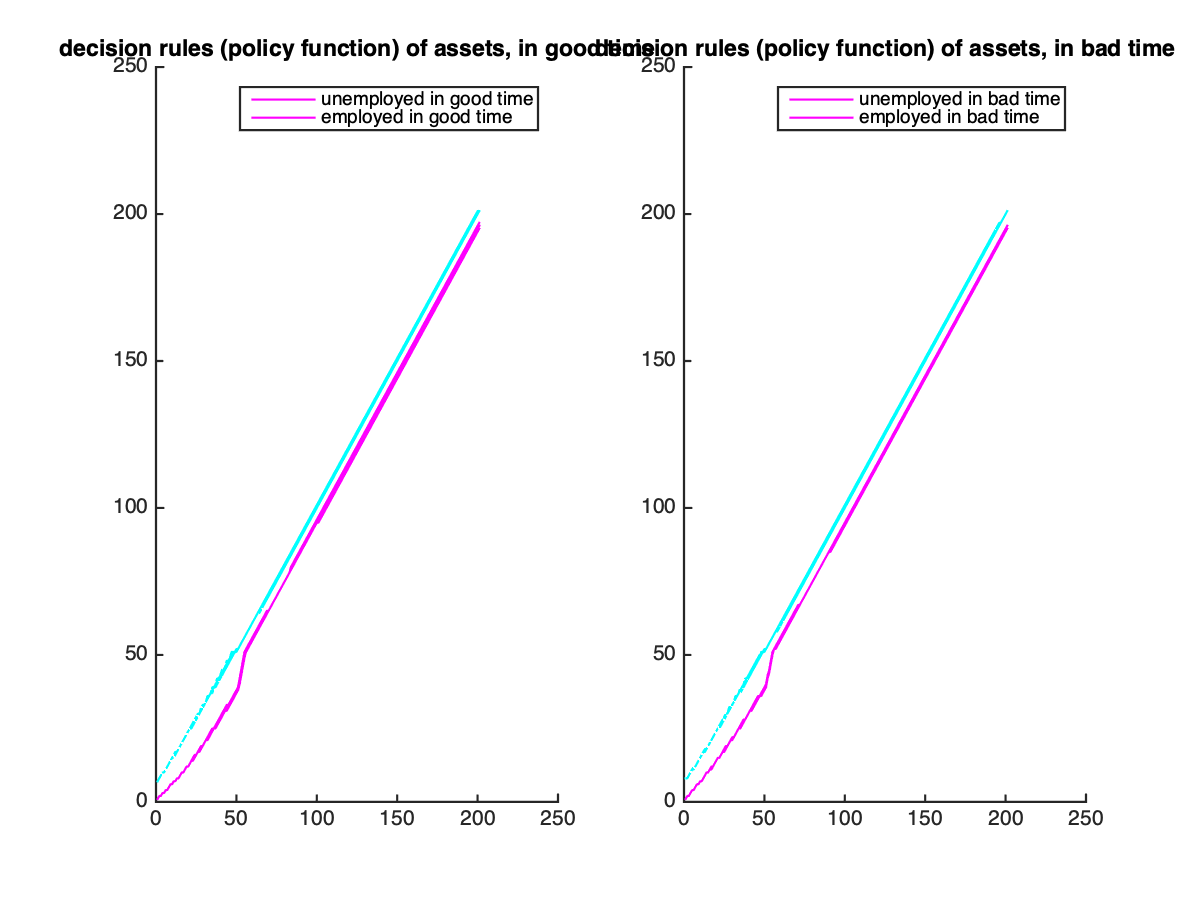
\includegraphics[width=\textwidth]{img/Q2_1_ab.png}
\caption{$a'(k,K,\epsilon,z,a)$}
\end{figure}


\subsection{Solution of the model}

the steps followed are illustrated inside the code as comments. 


\subsubsection{PEA}
I follow Luis's sample code, and output the graph of the policy function for assets below. 

Here I report the policy function w.r.t individual savings ($k$), given a fixed number of Aggregate capital ($K$), for different idiosyncratic shocks states. 
It can be seen that whenever good or bad productivity shocks are, employed is always better than unemployed, since a positive wage lead a higher saving. And since the difference between good and bad productivity shocks are not so huge, then, bad times savings is only slightly lower than good times'. 

\begin{figure}[htbp]
\centering
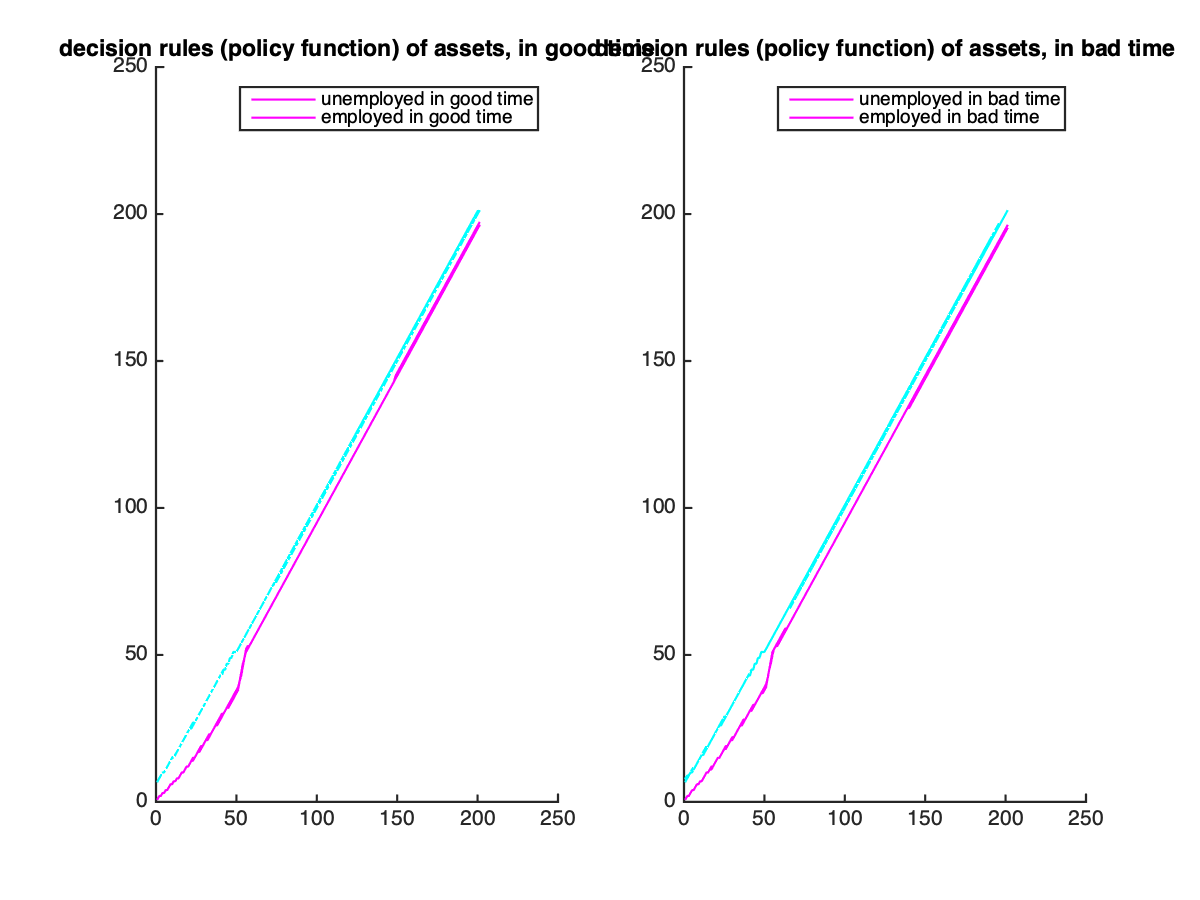
\includegraphics[width=\textwidth]{img/Q2_1_b.png}
\caption{$a'(k,K,\epsilon,z,a)$}
\end{figure}

\pagebreak
\subsection{Simulate the model for 2000 periods and 1000 individuals.}
\begin{figure}[htbp]
\centering
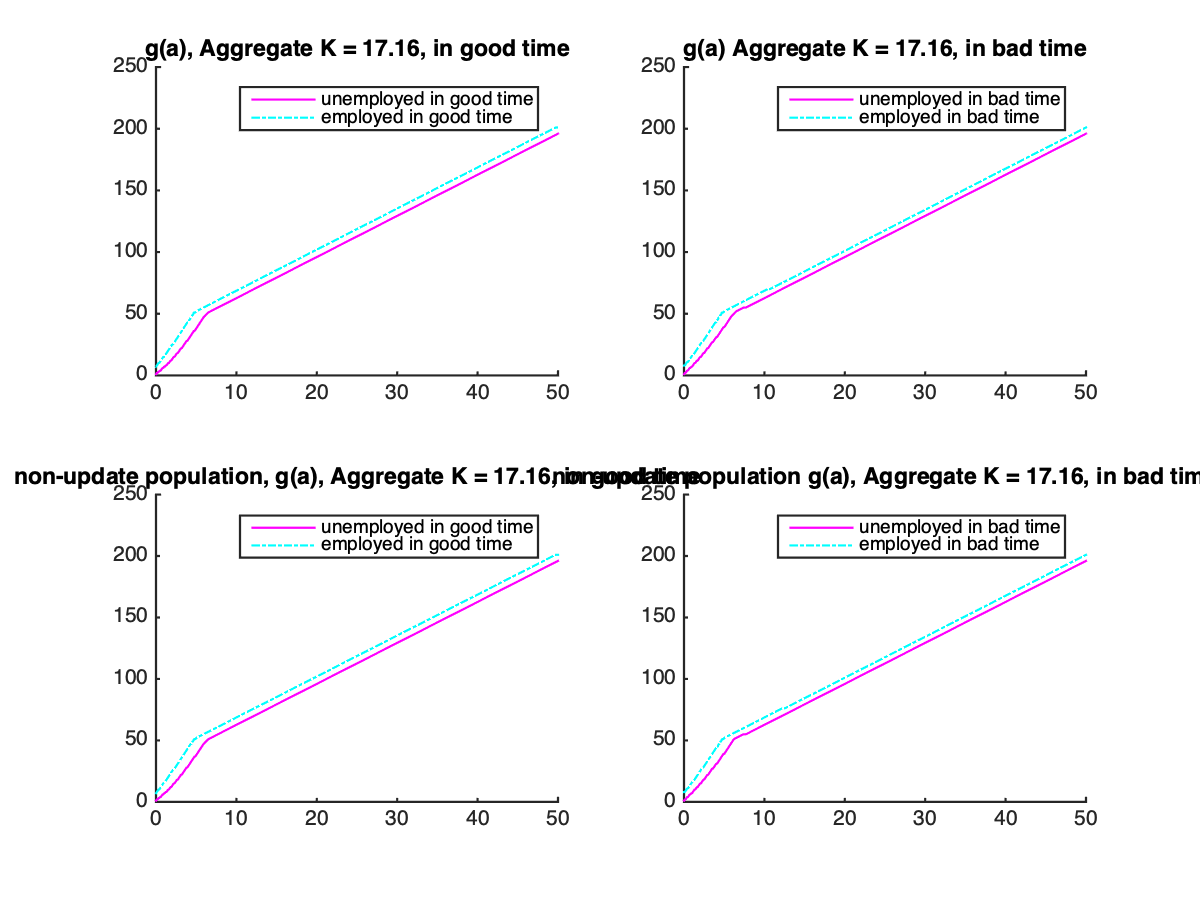
\includegraphics[width=\textwidth]{img/Q3_2_a.png}
\caption{$a'(k,K,\epsilon,z,a)$}
\end{figure}

\begin{figure}[htbp]
\centering
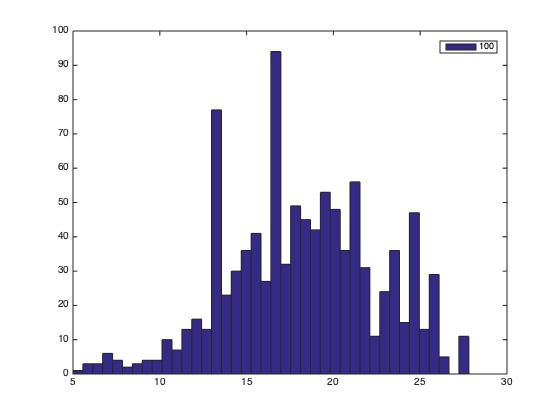
\includegraphics[width=\textwidth]{img/dist.png}
\caption{$Asset Distribution (final)$}
\end{figure}

\subsubsection{Compare the welfare of the agents that have the model with the best fit and the agents with the expectations that are never updated}

This part is in the matlab file: \textbf{3-2.m}

Total wealth of the agents never update will save slightly more than agents update their beliefs. Since the agents never update will adjust to save more for self-insurance schemes.

\begin{figure}[htbp]
\centering
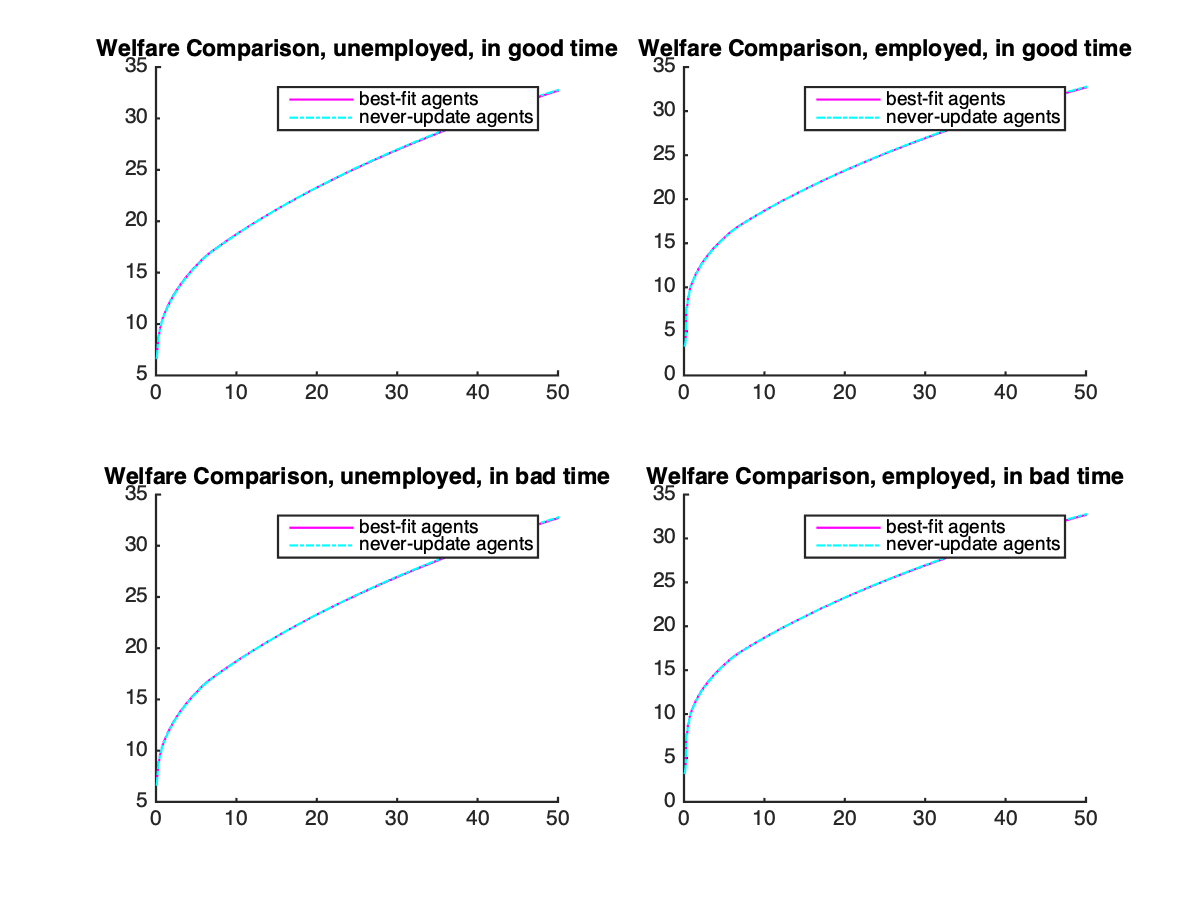
\includegraphics[width=\textwidth]{img/Q3_2_b.png}
\caption{Total welfare (as a function of initial wealth state)}
\end{figure}

\begin{figure}[htbp]
\centering
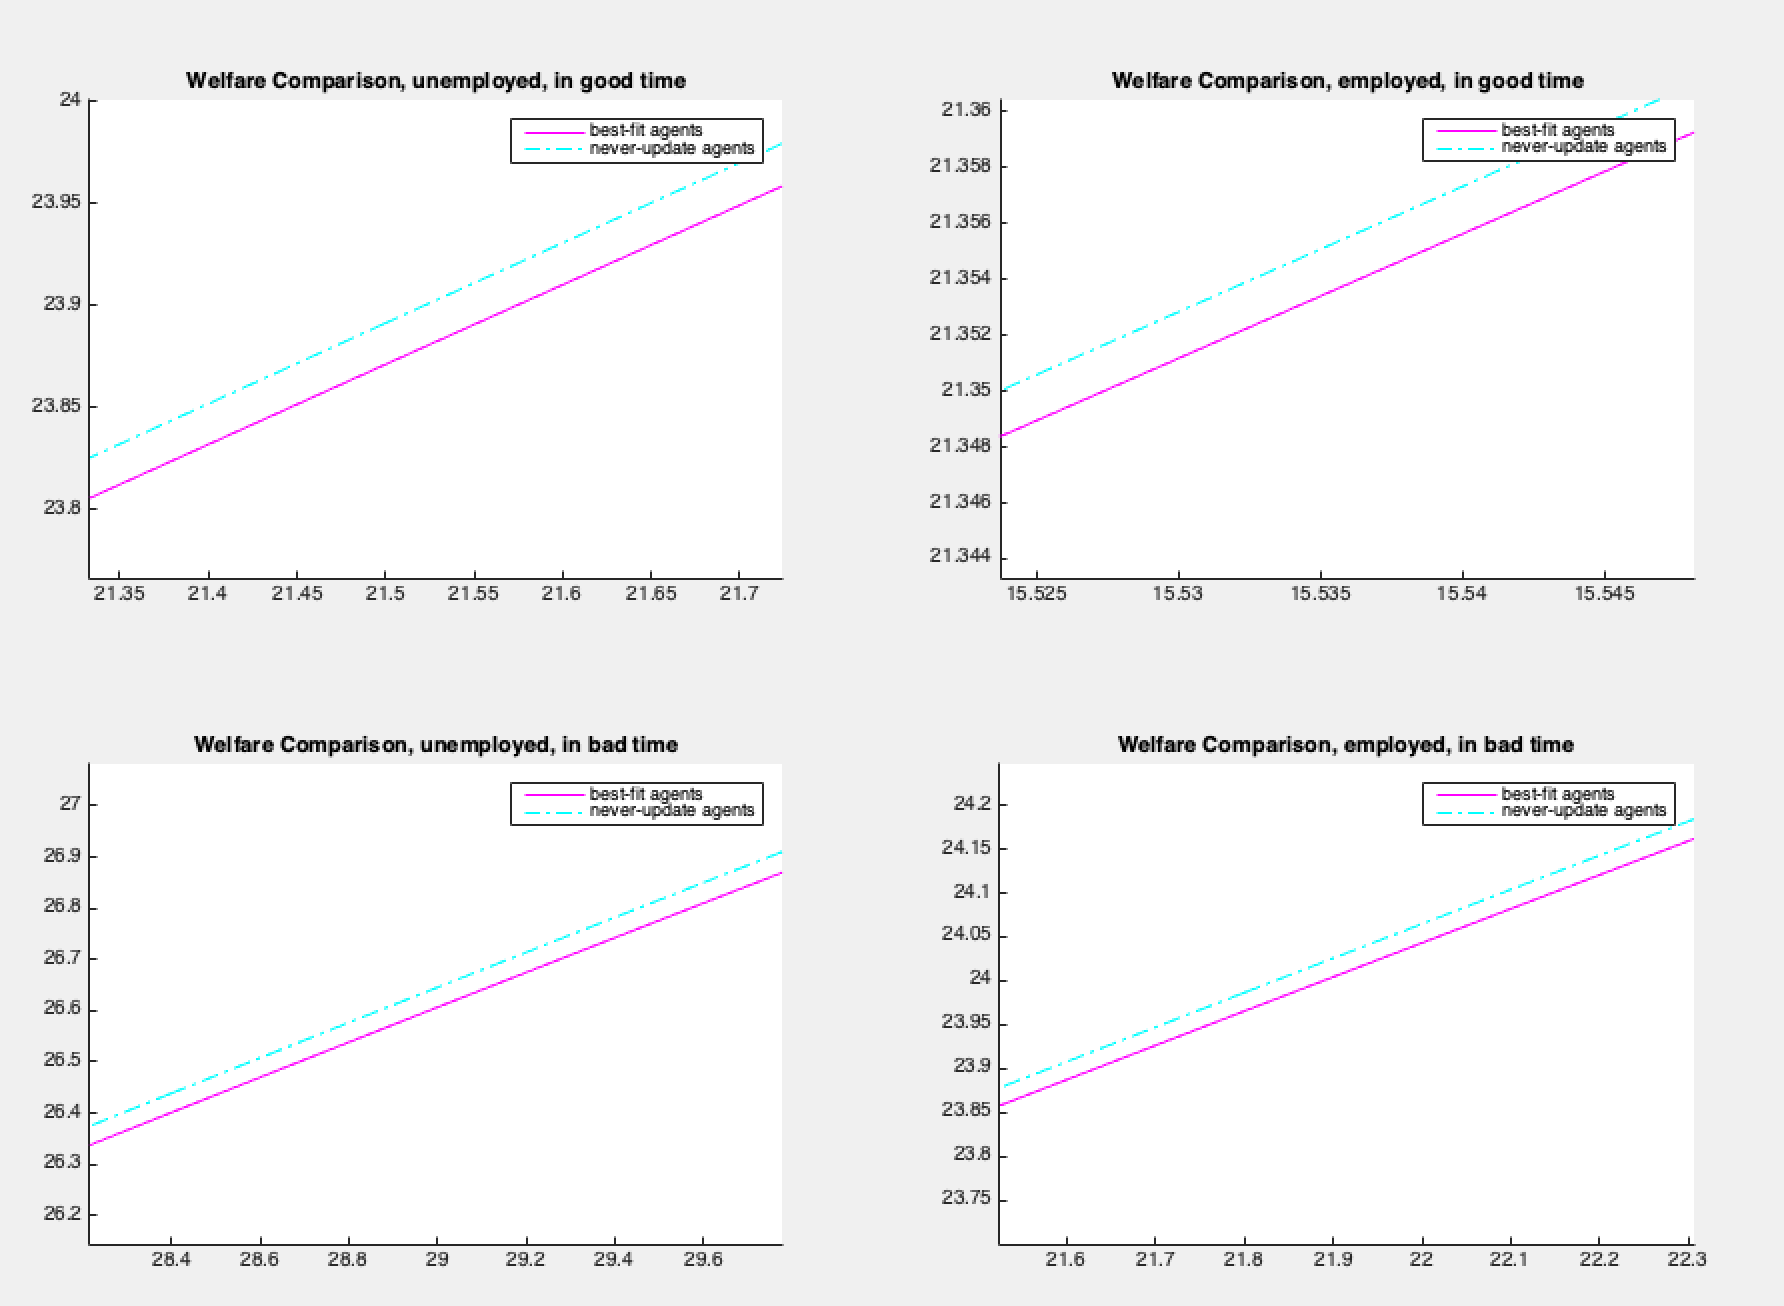
\includegraphics[width=\textwidth]{img/bigger.png}
\caption{Total welfare (as a function of initial wealth state)}
\end{figure}


%\begin{figure}[htbp]
%\centering
%\begin{minipage}[t]{0.48\textwidth}
%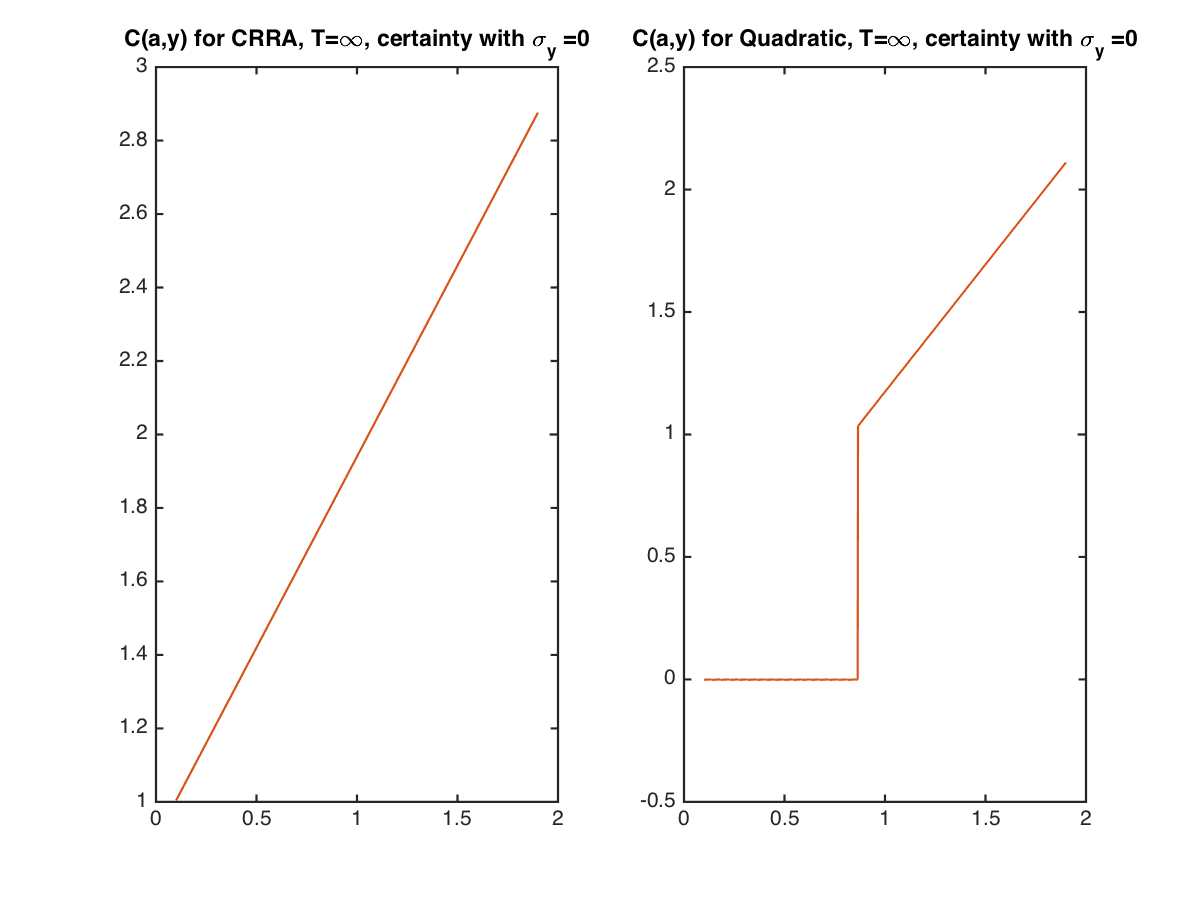
\includegraphics[width=\textwidth]{img/41a.png}
%\caption{$T=\infty, c(a,y)$ for two utility functions}\label{Fig1}
%\end{minipage}
%\begin{minipage}[t]{0.48\textwidth}
%\centering
%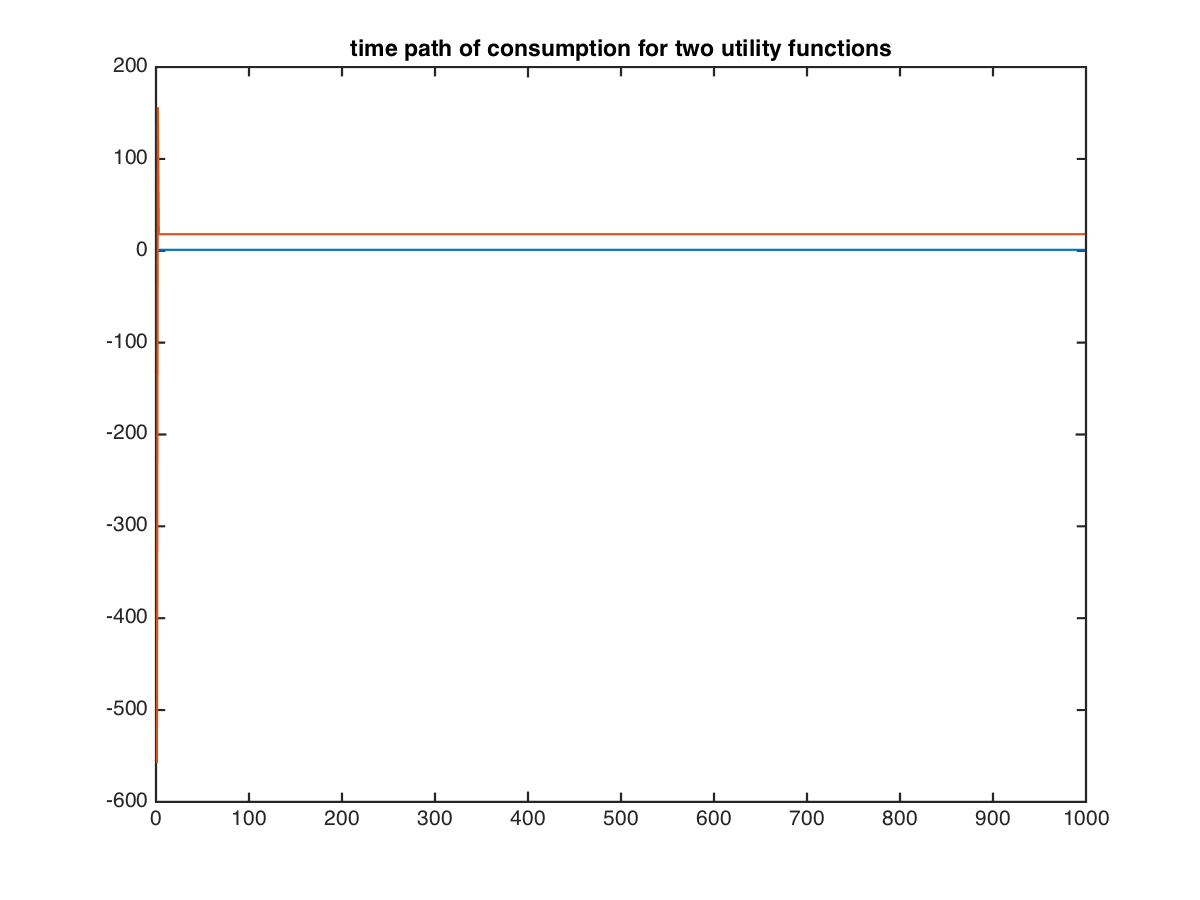
\includegraphics[width=\textwidth]{img/41aa.png}
%\caption{Q4-1b}\label{Fig2}
%\end{minipage}
%\end{figure}

















